\documentclass[10pt,UTF8]{ctexart}


\usepackage[margin=2cm,a4paper]{geometry}
%\usepackage[left=0.75in,top=0.6in,right=0.75in,bottom=1.0in,a4paper]{geometry}

\setmainfont{Caladea}
%% 也可以選用其它字庫:
% \setCJKmainfont[%
%   ItalicFont=AR PL KaitiM GB,
%   BoldFont=Noto Sans CJK SC,
% ]{Noto Serif CJK SC}
% setCJKsansfont{Noto Sans CJK SC}
% \renewcommand{\kaishu}{\CJKfontspec{AR PL KaitiM GB}}

% 繁體中文
\setCJKmainfont[Path=fonts/ ]{NotoSansTC-Medium.otf}

\usepackage{minted}
\usepackage[breaklinks]{hyperref}

% Picture
% 導言區的此三行無變化
\usepackage{graphicx}
\usepackage{float} 
\usepackage{subfigure}
% 以下是新增的自定義格式更改
\usepackage[]{caption2} %新增調用的宏包
\renewcommand{\figurename}{Fig.} %重定義編號前綴詞
\renewcommand{\captionlabeldelim}{.~} %重定義分隔符
 %\roman 是羅馬數字編號,\alph是默認的字母編號,\arabic是阿拉伯數字編號,可按需替換下一行的相應位置
\renewcommand{\thesubfigure}{(\roman{subfigure})}%此外,還可設置圖編號顯示格式,加括號或者不加括號
\makeatletter \renewcommand{\@thesubfigure}{\thesubfigure \space}%子圖編號與名稱的間隔設置
\renewcommand{\p@subfigure}{} \makeatother

% Math
\usepackage {mathtools}
\usepackage{amssymb}

% Code
\usepackage{listings}
\usepackage{xcolor}
\lstset{
    % backgroundcolor=\color{red!50!green!50!blue!50},
    % 程式碼塊背景色為淺灰色
    rulesepcolor= \color{gray}, % 程式碼塊邊框顏色
    breaklines=true,  % 程式碼過長則換行
    numbers=left, % 行號在左側顯示
    numberstyle= \small,% 行號字型
    % eywordstyle= \color{red,% 關鍵字顏色
    commentstyle=\color{gray}, % 註釋顏色
    frame=shadowbox % 用方框框住程式碼塊
    }

\usepackage{hyperref}

\title{算法分析和複雜性理論}
\author{干皓丞,2101212850, 信息工程學院}

\begin{document}
\maketitle


\section{作業目標與章節摘要}

求解遞推方程的四個例題(例 1 ~ 例 4)

1. 例題 1 : $T(n) =  9T(n/3) + n$

2. 例題 2 : $T(n) = T(2n /3) + 1$

3. 例題 3 : $T(n) = 3T(n/4) + n\log n$

4. 例題 4 : $T(n) = 2T( \frac{n}{2}) + n \log n $

\section{作業內容概述}

作業可以從 GitHub 下的 kancheng/kan-cs-report-in-2022 專案找到,作業程式碼與文件目錄為 kan-cs-report-in-2022/AATCC/lab-report/。實際執行的環境與實驗設備為 Google 的 Colab 、MacBook Pro (Retina, 15-inch, Mid 2014) 、 Acer Aspire R7 與 HP Victus (Nvidia GeForce RTX 3060)。

本作業 GitHub 專案為 kancheng/kan-cs-report-in-2022 下的 AATCC` 的目錄。程式碼可以從 code 目錄下可以找到 *.pynb,內容包含上次課堂練習、LeetCode 範例思路整理與作業。

https://github.com/kancheng/kan-cs-report-in-2022/tree/main/AATCC

\begin{figure}[H]
\centering 

\includegraphics[width=0.30\textwidth]{aatccqr.png} 
\caption{作業專案位置}
\label{Test}
\end{figure}

1. LeetCode : https://leetcode.com/

2. LeetCode CN : https://leetcode-cn.com/

3. OnlineGDB : https://www.onlinegdb.com/ 

LeetCode 的平台部分, CN 的平台有針對簡體中文使用者進行處理,包含中英文切換等功能。OnlineGDB 則可線上進行簡易的環境測試,其程式碼涵蓋 C, C++, C\#, Java, Python, JS, Rust, Go。

\newpage

\section{作業推導}

\begin{figure}[H]
\centering 
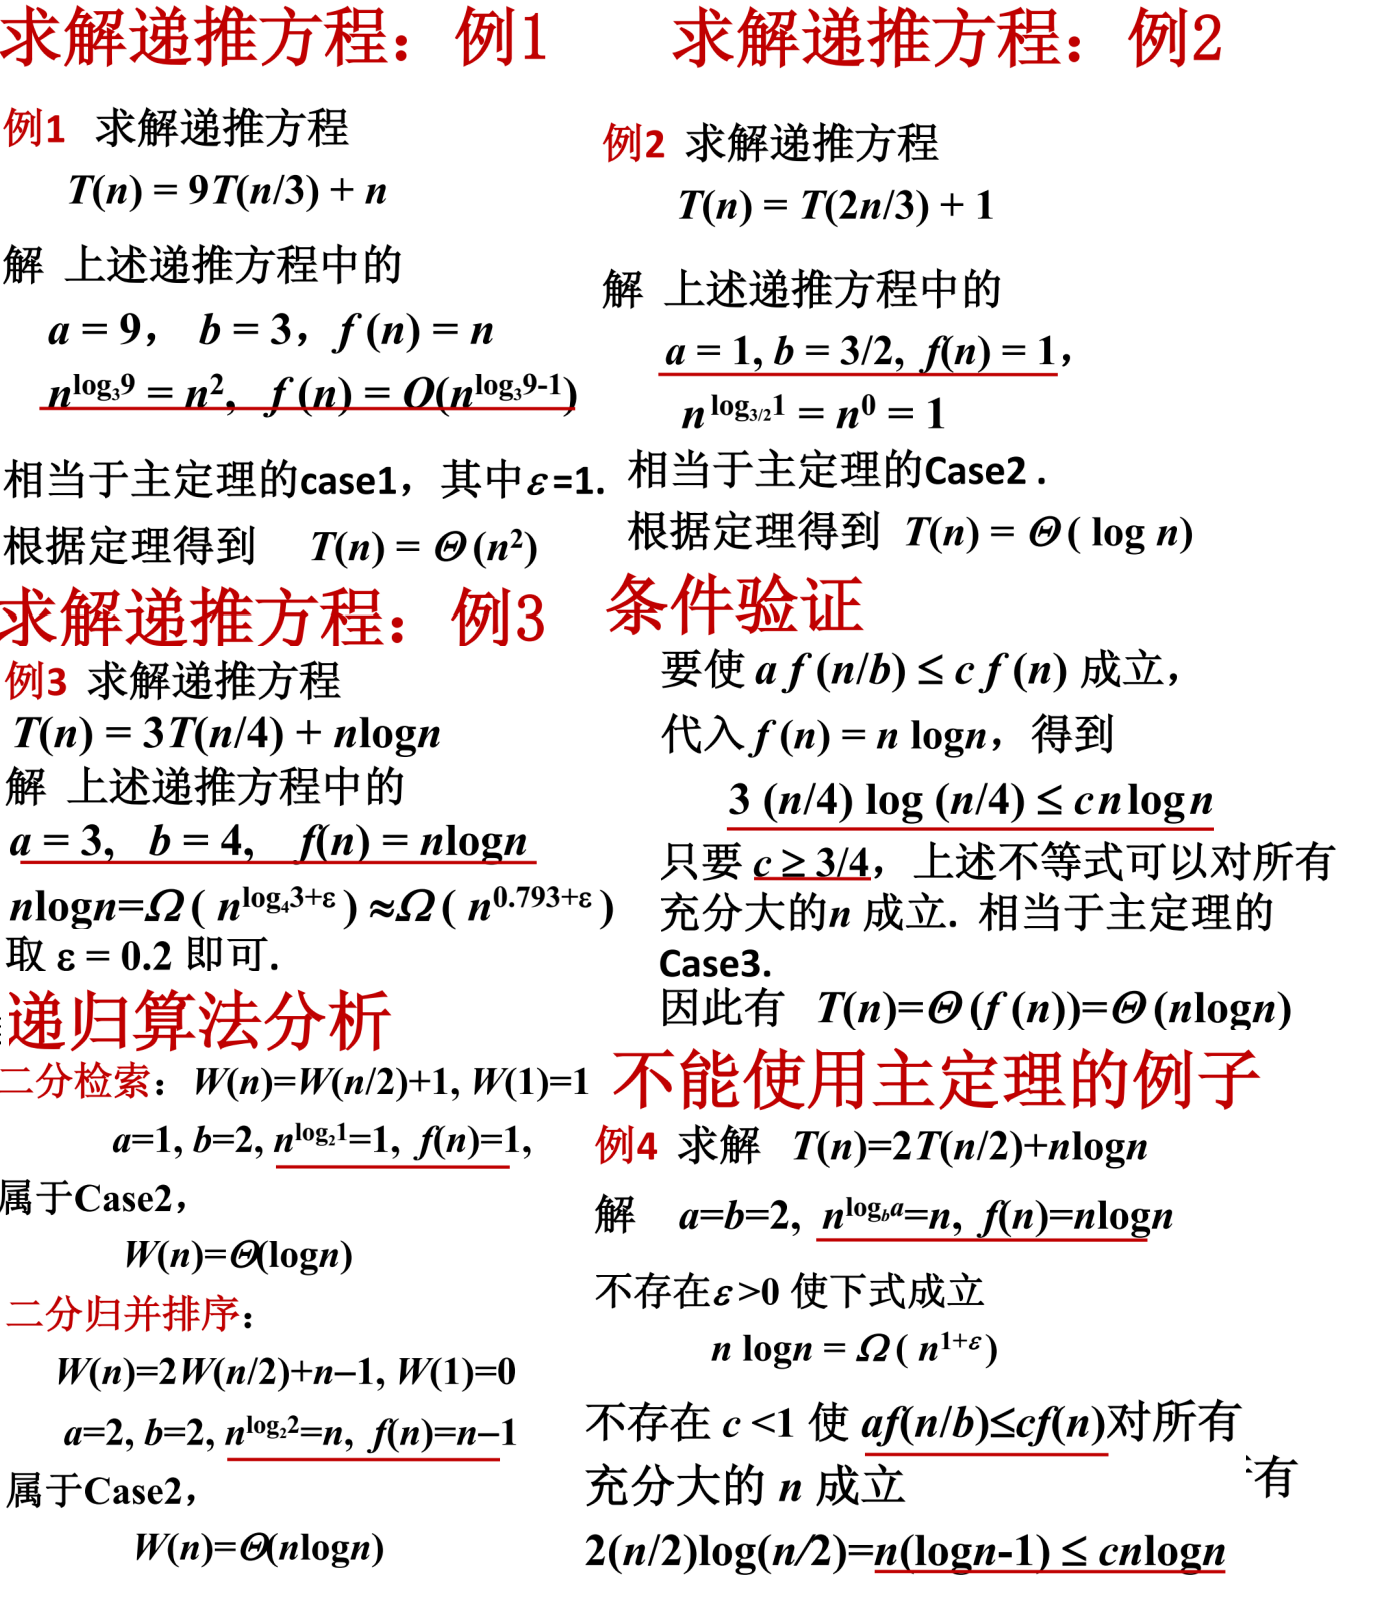
\includegraphics[width=0.95\textwidth]{w14-kp-27.png} 
\caption{課程內容}
\label{Test}
\end{figure}

\subsection{例題 1}

$T(n) =  9T(n/3) + n$

由主定理 $a = 9, b = 3$

$\log_b a = 2 $

$\exists  \varepsilon > 0 s.t. f(n) = n = O(n^{2 - \varepsilon})$

$\therefore 由於情況 1, T(n) = \Theta(n^{2}) $

\subsection{例題 2}

$T(n) = T(2n /3) + 1, a = 1, b = 3/2, \log_b a = 0$

$f(n) = 1 = n^{0} = \Theta(n^{2})$

$\therefore 由於情況 2, T(n) = \Theta(n^{0} \log n) = \Theta(n) $

\subsection{例題 3}

$T(n) = 3T(n/4) + n\log n, a = 3, b = 4, \log_b a = \log_4 3 < 1$

$f(n) = n\log(n) = \Omega(n) = \Omega(n^{\log_4 3 + (1 - \log_4 3)})$

且 $\exists c < 1, \exists n_{0}  s.t. \forall n > n_{0}, 3f(n/4) = \frac{3n}{4}\log {\frac{n}{4}} \leq cn\log n$

$(取 c = \frac{7}{8} 即可滿足) \therefore 由於情況 3, T(n) = \Theta(n \log n) = \Theta(n) $

\subsection{例題 4}

$T(n) = 2T( \frac{n}{2}) + n \log n $,

$ a = 2, b = 2, \log_b a = 1$

$f(n) = n \log n = \Omega(n^{1+\varepsilon})$

而顯然 $ \nexists c < 1, s.t. \exists n_{0}, \forall n > n_{0}, n \log \frac{n}{2} \leq c n \log n$

$ \therefore $ 主定理失效,以下用無窮級數處理 : 

$ T(n) = 2T(\frac{n}{2} + n \log n = 4T (\frac{n}{4}) + n \log n + 2 \frac{n}{2} \log \frac{n}{2} $

$ = 8T(\frac{n}{8} + n \log n + 2 \frac{n}{2} \log \frac {n}{2} + 4 \frac{n}{4} \log \frac{n}{4}) = ... $

$ = n \log n + n \log \frac{n}{2} + n \log \frac {n}{4} + ... =  $

$ = n (  \log n + \log n - 1 + \log n - 2 + \log n - 3 + ... + 0 ) $

$ = \Theta(n \log^{2} n) $






%\section{附錄}

% 數學意義說明

% $$\min \limits_{G}\max \limits_{D}{V_I(D,\ G)=V(D,G)-\lambda L_I(G,Q)}$$

%	\begin{lstlisting}[language={python}]

%	\end{lstlisting}

%\begin{enumerate}
%\item Y
%\item A
%\end{enumerate}

% \newpage

\clearpage

\end{document}